%
% Libro online bastante completo para consulta de Latex: http://en.wikibooks.org/wiki/LaTeX/
% Versión en castellano: http://es.wikibooks.org/wiki/Manual_de_LaTeX
\documentclass[12pt, a4paper, titlepage]{article}

\usepackage[spanish]{babel} % Soporte multilenguaje para LaTeX.

\usepackage[a4paper, top=2.5cm, bottom=2.5cm, left=2.5cm, right=2.5cm]{geometry} % Interfaz flexible para definir las dimensiones del documento

\usepackage[utf8]{inputenc} % Aceptar diferentes tipos de codificación de caracteres de entrada (en este caso usamos la codificación Unicode UTF-8)

\usepackage{graphicx} % Soporte aumentado para gráficos 
\usepackage{hyperref} % Para manejar referencias cruzadas. P.ej. añadir hiperenlaces al índice
\usepackage{rotating}

\begin{document}

%%%%%%%%%%%%%%%%%%%%%%%%%%%%%%%%%%%%%%%%%%%%%%%%%%%%%%%%%%%%%%%%%%%%%%%%%%%%%%%%
% PORTADA
%%%%%%%%%%%%%%%%%%%%%%%%%%%%%%%%%%%%%%%%%%%%%%%%%%%%%%%%%%%%%%%%%%%%%%%%%%%%%%%%

\begin{titlepage}


\includegraphics[width=15cm]{Imagenes/Simbolo_logo_UDC.png}

% Lista de tamaños: \Huge, \huge, \LARGE, \Large, \large, \small, \footnotesize, \tiny
\vspace{3cm}

\begin{center}

\includegraphics[scale=0.3]{Imagenes/1a_Practica_ER_14-15.png}
\end{center}

\begin{flushright}
	\LARGE{\textbf{ JoinMe!}}\\
	\LARGE{\textbf{Especificación de casos de uso}}\\
	\large{\textbf{Version 1.3}}
	
		
\end{flushright}
\vspace{1cm}
\begin{center}
José Antonio López Sebio\\
Pablo Paz Varela\\
Grupo ER-12-03\\
\end{center}

\vspace{2cm}
\begin{center}
	\large{\textbf{Histórico}}
	
    \begin{tabular}{ | p{4cm} | p{2cm} | p{5cm} | p{4cm} |}
    \hline
    \textbf{Date} & \textbf{Version} & \textbf{Description} & \textbf{Author} \\ \hline
    04/03/2014 & 1.0 & Borrador 1  & ER-12-03  \\ \hline
     04/03/2014 & 1.1 & Añadadida resumen casos de uso & ER-12-03  \\ \hline
     06/03/2014 & 1.2 & Añadidos casos de uso detallados & ER-12-03  \\ \hline
     06/03/2014 & 1.3 & Añadidos diagramas & ER-12-03  \\ \hline
    \end{tabular}
\end{center}

\end{titlepage}
\clearpage

%%%%%%%%%%%%%%%%%%%%%%%%%%%%%%%%%%%%%%%%%%%%%%%%%%%%%%%%%%%%%%%%%%%%%%%%%%%%%%%%
% INDICE
%%%%%%%%%%%%%%%%%%%%%%%%%%%%%%%%%%%%%%%%%%%%%%%%%%%%%%%%%%%%%%%%%%%%%%%%%%%%%%%%

\tableofcontents
\clearpage

%%%%%%%%%%%%%%%%%%%%%%%%%%%%%%%%%%%%%%%%%%%%%%%%%%%%%%%%%%%%%%%%%%%%%%%%%%%%%%%%
\section{Introducción}
%%%%%%%%%%%%%%%%%%%%%%%%%%%%%%%%%%%%%%%%%%%%%%%%%%%%%%%%%%%%%%%%%%%%%%%%%%%%%%%%

El objetivo de este documento es mostrar una breve descripción de la red social \textbf{JoinMe!} y describir los actores conocidos y su interacción con el sistema.
Este documento muestra una visión de alto nivel, además de una visión más detallada de los casos de uso más importantes.

%%%%%%%%%%%%%%%%%%%%%%%%%%%%%%%%%%%%%%%%%%%%%%%%%%%%%%%%%%%%%%%%%%%%%%%%%%%%%%%%
\section{Actores}
\begin{description}

\item [Usuario] Usuario que inicia sesión dentro del sistema, para estar en contacto con sus amigos, participar en grupos, compartir fotos/ficheros/videos...

\item [Empresa] Usuario que representa a una empresa e inicia sesión dentro del sistema para gestionar sus anuncios.

\end{description}
%%%%%%%%%%%%%%%%%%%%%%%%%%%%%%%%%%%%%%%%%%%%%%%%%%%%%%%%%%%%%%%%%%%%%%%%%%%%%%%%


%%%%%%%%%%%%%%%%%%%%%%%%%%%%%%%%%%%%%%%%%%%%%%%%%%%%%%%%%%%%%%%%%%%%%%%%%%%%%%%%
\section{Resumen de casos de uso}
%%%%%%%%%%%%%%%%%%%%%%%%%%%%%%%%%%%%%%%%%%%%%%%%%%%%%%%%%%%%%%%%%%%%%%%%%%%%%%%%

\begin{description}
    \item [CU01 - Registrar usuario]: Para que un usuario pueda utilizar las funcionalidades que ofrece la red social \textbf{JoinMe!} tiene que registrarse, bien proporcionando sus datos reales o bien un certificado digital
o el DNIe. Pero siempre necesario un email y contraseña.
   	\item [CU02 - Modificación de perfil]: Un usuario registrado puede querer modificar alguno de los datos almacenados en la red social, como puede ser su email o contraseña.
    \item [CU03 - Aceptar solicitud de amistad]: Los usuarios regristrados pueden aceptar las solicitudes de amistad enviadas por otros usuarios. Estas solicitudes aparecerán en un área de notificaciones.
    
    \item [CU04 - Rechazar solicitud de amistad]: Los usuarios regristrados pueden rechazar las solicitudes de amistad que consideren oportunas y que tienen disponibles en el área de notificaciones.
    
    \item [CU05 - Ver amigos]: Un usuario registrado puede consultar los amigos accediento a la lista de los mismos. Haciendo click en el nombre de usuario, accederá al perfil del mismo.
    
    \item [CU06 - Enviar solicitud de amistad]: Accediendo al perfil de un usuario después de haberlo buscado mediante el buscador, o bien por acceso directo mediante un link, el visitante puede enviar una petición de amistad haciendo click en el botón oportuno.
    
    \item [CU07 - Crear círculo]: Los usuarios registrados pueden crear círculos para organizar sus amistades. En la creación del círculo es necesario introducir un nombre para el círculo y voluntariamente una descripción.
    
    \item [CU08 - Borrar círculo]: Los usuarios pueden borrar los círculos que estimen oportunos sin afectar a las amistades que tengan incluídas en ellos.
    
	\item [CU09 - Añadir amigo a círculo]: Los usuarios pueden incluir amigos en sus círculos, bien mediante un formulario donde intrucirán el nombre del amigo, o bien desde el perfil de su amigo donde existirán un botón \textbf{Añadir a círculo} que mostrará un desplegable con los círculos existentes y la posibilidad de crear uno nuevo.
	
	\item [CU10 - Eliminar amigo de un círculo]: Los usuarios pueden eliminar amigos de los círculos, para ello tienen que acceder al círculo en cuestión y eliminar al amigo.
	
	\item [CU11 - Cambiar frase de estado]: Los usuarios podrán cambiar su frase de estado las veces que estimen oportuno, para ello existirá un formulario con una entrada de texto donde el usuario tendrá que escribar la frase, y un botón para el envío de la misma.
	
	\item [CU12 - Publicar acción en el muro]: Las acciones realizadas por el usuario registrado serán publicadas en el muro. Este caso de uso representa la publicación de cualquier acción en el muro (subida de fotografía/video, cambio de frase de estado, aceptación de petición de amistad, etc.).
	
	\item [CU13 - Crear entrada]: Los usuarios registrados pueden crear una entrada que se verá reflejada en su muro. Esta entrada puede incluir fotografías, enlaces, videos y texto, apareciendo cada uno de ellos de una manera concreta, por ejemplo, el enlace incluíra una pequeña previsualización de texto e imágenes en el caso de que las contenta. Las imágenes tendrá una previsualización al igual que los vídeos.
	
	\item [CU14 - Borrar entrada]: Los usuarios peuden borrar las entradas que crearon anteriormente, para ello tienen que hacer click en el botón correspondiente.
	
	\item [CU15 - Editar entrada]: Los usuarios pueden editar el texto y los elementos de una entrada creada anteriormente.
	
	\item [CU16 - Crear grupo]: Los usuarios registrados pueden crear un grupo para unir a personas afines al interés del grupo, para ello existirán un formulario accesible desde la página principal, donde el usuario, en adelante administrador del grupo, introducirá nombre y descripción y podrá invitar a sus contactos a unirse al mismo.
	
	\item [CU17 - Eliminar grupo]: El admistrador del grupo tiene la posibilidad de eliminar el mismo, con lo cual el grupo dejaría de existir y todos los miembros dejarían de serlo.
	
	\item [CU18 - Ingresar en un grupo]: Un usuario registrado puede acceder a un grupo, para ello tiene que hacer click en el botón de Ingresar en grupo presente en la página principal del grupo.
	
	\item [CU19 - Salir de un grupo]: Un usuario registrado miembro de un grupo puede salir, para ello tienen que hacer uso del botón Salir del grupo.
	
	\item [CU20 - Publicar noticia en un grupo]: Los grupos cuentan con un grupo donde los usuarios miembros podrań publicar notícias al igual que pueden publicarlas en su muro, creando las mismas previsualizaciones para los enlaces, vídeos...
	
	\item [CU21 - Crear hilo en un foro de discusión de grupo]: Los grupos disponen de un foro de discusión, donde los miembros podrán crear un hilo de discusión al hacer click en el botón correspondiente y rellenando el formulario con título, y una caja de texto donde intrudirá el texto de la discusión.
	
	\item [CU22 - Responder en un hilo del grupo]: Todo hilo del foro de discusión de un grupo puede tener respuestas mientras este siga abierto, para que el usuario puede crear una respuesta tiene que hacer uso del botón correspondiente de \textbf{Responder} y cubrir el formulario.
	
	\item [CU23 - Crear álbum de fotografías]: Los usuarios registrados pueden crear álbumes para tener organizadas sus fotografías, para ello desde su perfil tendrán un botón que les dará acceso a un formulario con título del álmbum y una descripción voluntaria, así como más datos de información.
	
	\item [CU24 - Subir fotografía]:  Los usuarios registrados pueden subir una fotografía y asignarla a uno de sus álbumes creados o no. 
	
	\item [CU25 - Borrar álbum de fotografías]: Los usuarios registrados pueden borrar los álbumes creados. Para ello tienen que acceder al álbum en cuestión y hacer uso del botón \textbf{Eliminar álbum}.
	
	\item [CU26 - Borrar fotografía]: Las fotografías subidas también pueden ser borradas, para ello cada fotografía contará con un botón para realizar esta acción.
	
	\item [CU27 - Etiquetar contacto en fotografía]: En cada fototgrafía existirá la opción de etiquetar a tus amigos, para que se más fácil reconocerlos por otras personas.
	
	\item [CU28 - Borrar etiqueta de fotografía]: Las etiquetas existentes en una fotografía pueden ser eliminadas, para ello el usuario tiene que ver todas las etiquetas y eliminar las que le interese.
	
	\item [CU29 - Edición sencilla de fotos]: La red social \textbf{JoinMe!} cuenta con un pequeño editor de fotos. Para editar las fotos, el usuario puede ir a la foto ya subida, o bien después de subirla se le dará la opción de editarla. Esta edición permite corregir defectos de brillo, contraste y otros características básicas de una imagen.
	
	\item [CU30 - Subir vídeo]: Los usuarios pueden subir vídeos, para ello tienen que seguir el mismo procedimiento que para subir una fotografía.
	
	\item [CU31 - Borrar vídeo]: Los usuarios puede eliminar los vídeos subidos anteriormente, para ello cada video tiene un botón para realizar esta acción.
	
	\item [CU32 - Comentar una publicación]: Las publicaciones pueden ser comentadas, bien por el usuario autor de la publicación o bien por los usuarios que pueden leer esa publicación. Para ello cada publicación dispone de un formulario y su correspondiente botón para enviar este comentario.
	
	\item [CU33 - Borrar comentario]: Los comentarios creados en una publicación pueden ser borrados, para ello el autor del comentario tiene que pulsar en el botón correspondiente en el comentario.
	
	\item [CU34 - Enviar mensaje privado]: La red social dispone de un sistema de Chat/Mensajes privados para la comunicación entre amigos. Para hacer uso de esta funcionalidad la res social dispone de un menú lateral de chat donde aparecerán los usuarios que están logueados en el sistema, donde pulsando en el nombre del contacto se abrirá una ventana de chat con su correspondiente caja de texto y botón de enviar mensaje. Otra opción para enviar un mensaje es visitar el perfil de contacto donde existirá un botón \textbf{Enviar mensaje privado}, que abrirá un formulario de envio de mensaje privado.
	
	\item [CU35 - Mostrar página de início]: Los usuarios tendrán una página de inicio donde verán todas las actividades relacionadas con sus amigos y grupos.
	
	\item [CU36 - Filtrar información en página de início]: La página de inicio tiene una serie de filtros donde los usuarios podrán filtrar la información que quieren ver por categoría. Para usar los filtros los usuarios tienen que seleccionar que categorías quieren ver.
	
	\item [CU37 - Subir ficheros]: Los usuarios tendrán disponible un formulario para subir ficheros a la red social.
	
	\item [CU38 - Borrar ficheros]: Los usuarios tendrán disponibles una página de gestión de ficheros subidos, donde podrán eliminar los subidos.
	
	\item [CU39 - Comprar \textit{JoinMe! Coins}]: Desde el perfil del usuario podrá acceder a una página para poder comprar la moneda de la red social, para ello tendrá que seleccionar que cantidad de \textit{JoinMe! Coins} quiere comprar mediante un formulario y seleccionar el método de pago.
	
	\item [CU40 - Regalar \textit{JoinMe! Coins}]: Desde el apartado de gestión de \textit{JoinMe! Coins} el usuario podrá hacer transfrencias del dinero virtual a sus contactos.
	
	\item [CU41 - Consultar catálogo de productos]: Existirá un enlace para consultar todos los productos que se pueden comprar con la moneda virtual de la red social.
		
	\item [CU42 - Comprar un producto]: Desde el catálogo de productos, el usuario podrá acceder a un producto en concreto y comprar pulsando el botón correspondiente después de seleccionar el número de unidades que desea.
	
	\item [CU43 - Indicar relevancia de un anuncio]: Los usuarios registrados pueden seleccionar la relevancia de los anuncios que les aparecen mientras navegan por la red social.
	
	\item [CU44 - Crear un anuncio]: Una empresa anunciadora registrada en la red social puede crear anuncios y asignarlos a una categoría estándar, para ello tiene que iniciar sesión y rellenar el formulario con los datos correspondientes al anuncio.
	

\end{description}


%%%%%%%%%%%%%%%%%%%%%%%%%%%%%%%%%%%%%%%%%%%%%%%%%%%%%%%%%%%%%%%%%%%%%%%%%%%%%%%%
\section{Diagramas}
%%%%%%%%%%%%%%%%%%%%%%%%%%%%%%%%%%%%%%%%%%%%%%%%%%%%%%%%%%%%%%%%%%%%%%%%%%%%%%%%
\begin{center}

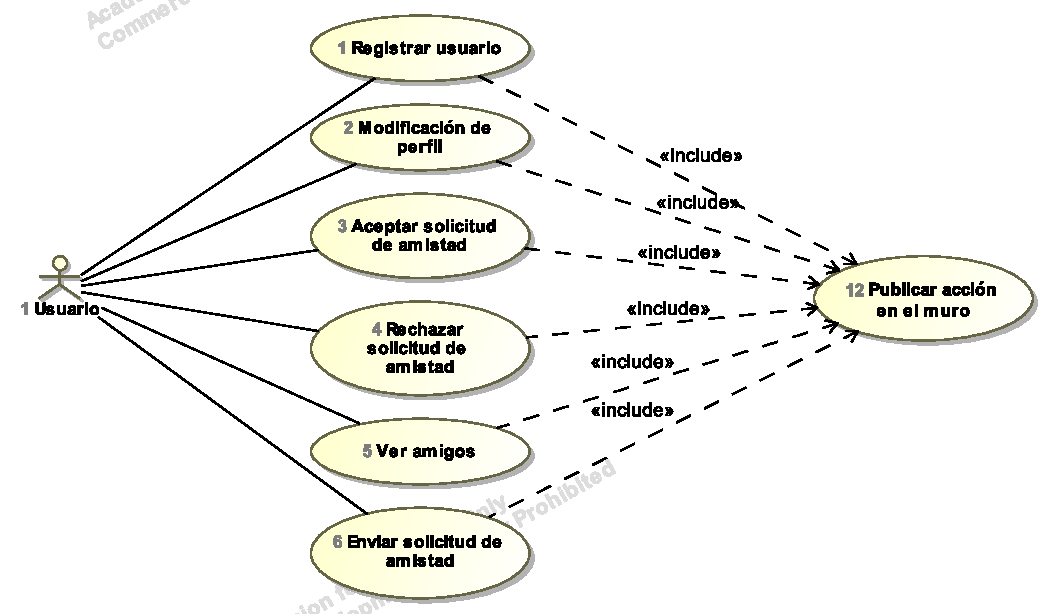
\includegraphics[width=\textwidth]{Imagenes/casosUso1}
\end{center}

\begin{center}
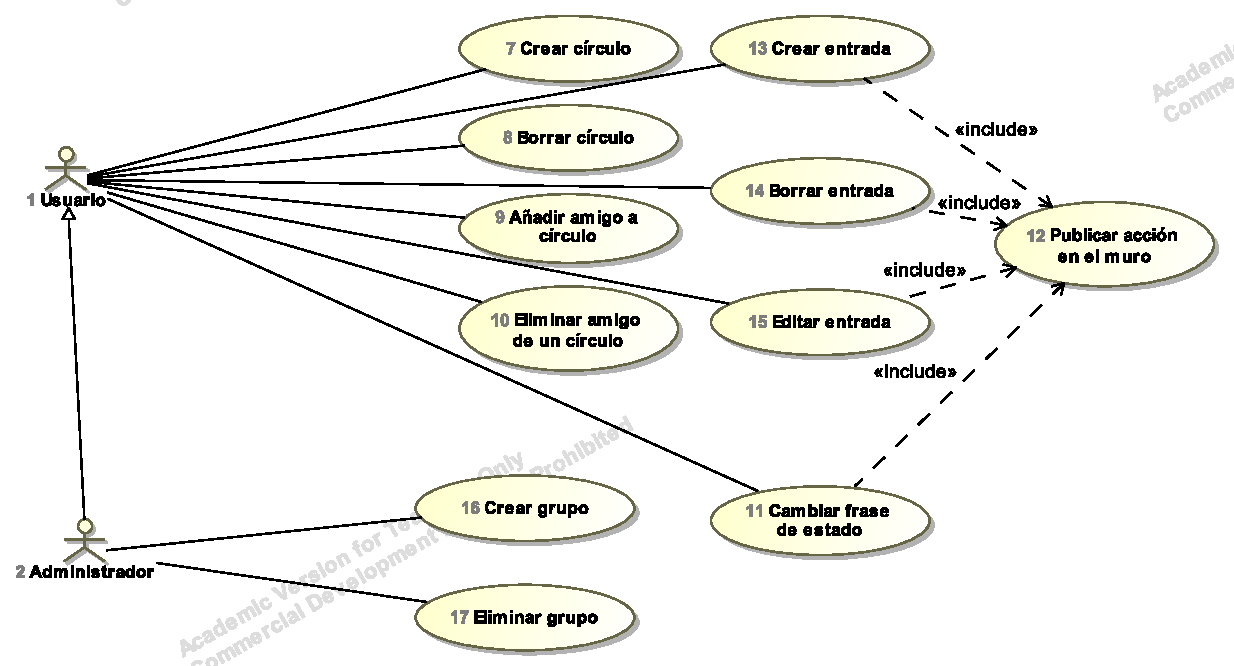
\includegraphics[width=\textwidth]{Imagenes/casosUso2}
\end{center}

\begin{center}
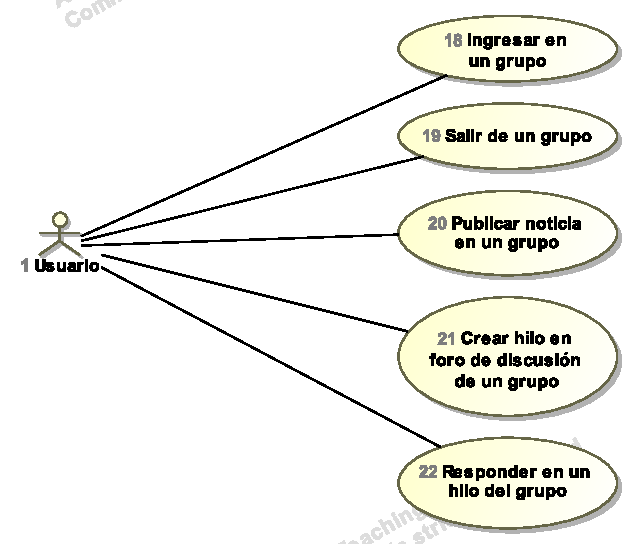
\includegraphics[scale=0.95]{Imagenes/casosUso3}
\end{center}

\begin{center}
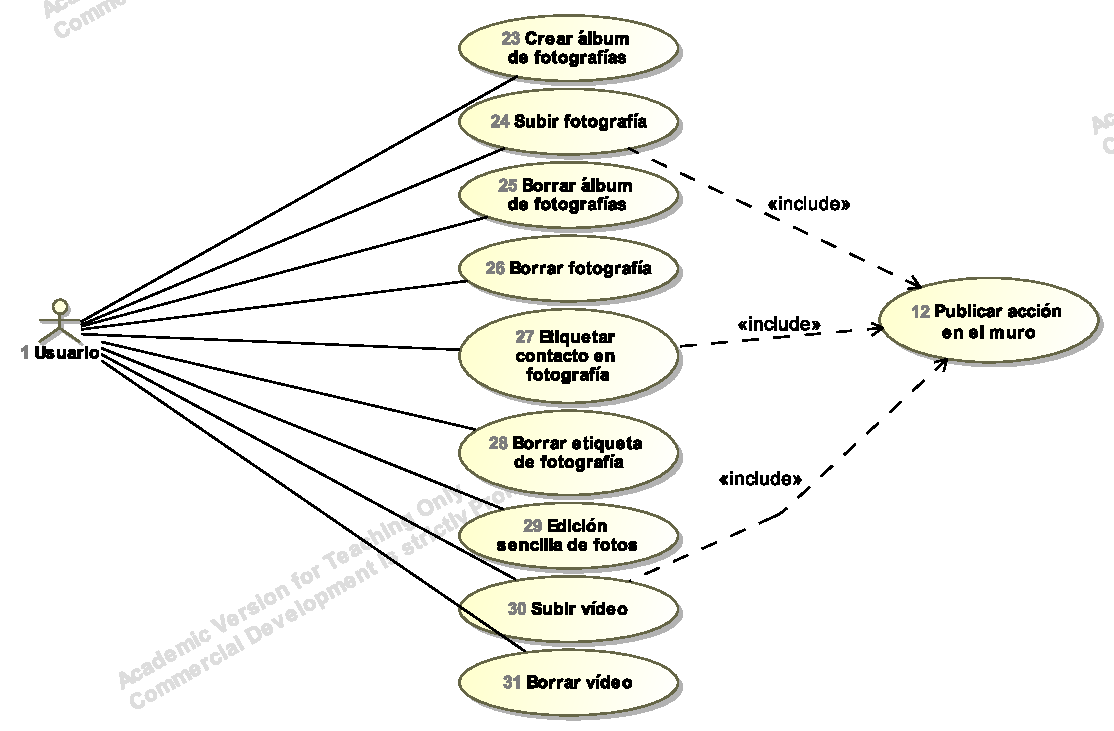
\includegraphics[width=\textwidth]{Imagenes/casosUso4}
\end{center}

\begin{center}
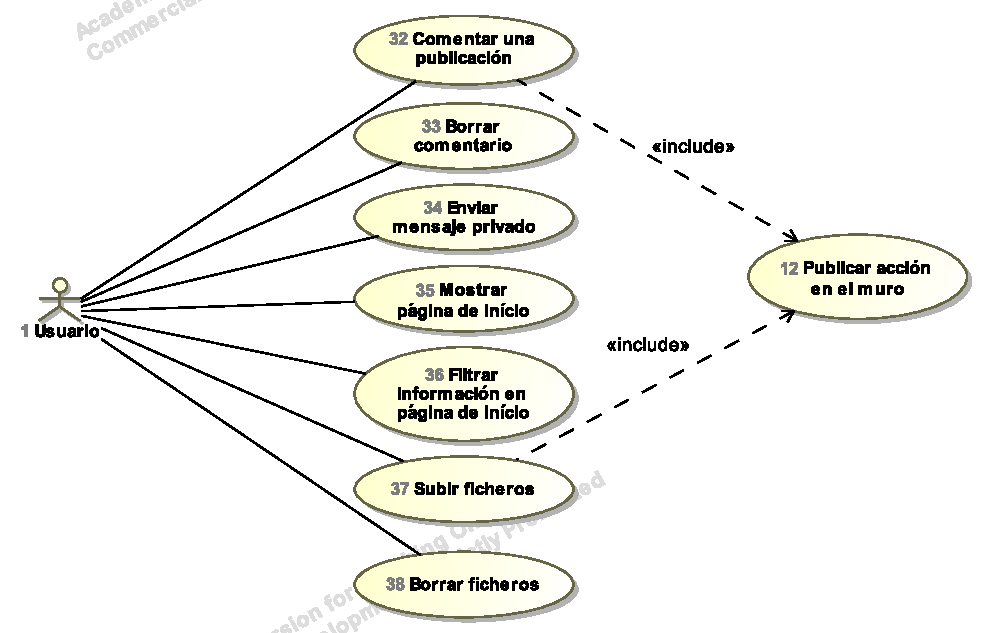
\includegraphics[width=\textwidth]{Imagenes/casosUso5}
\end{center}

\begin{center}
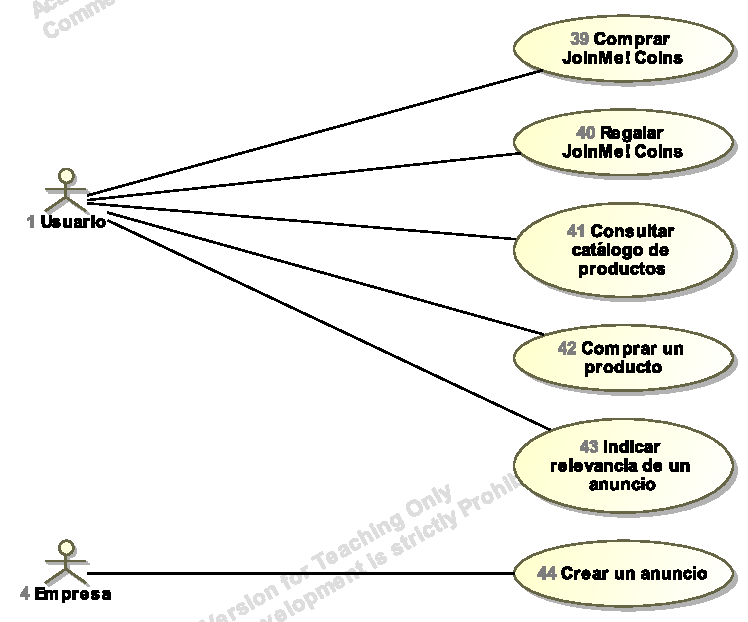
\includegraphics[scale=0.9]{Imagenes/casosUso6}
\end{center}

\newpage






%%%%%%%%%%%%%%%%%%%%%%%%%%%%%%%%%%%%%%%%%%%%%%%%%%%%%%%%%%%%%%%%%%%%%%%%%%%%%%%%
\section{Casos de Uso}
%%%%%%%%%%%%%%%%%%%%%%%%%%%%%%%%%%%%%%%%%%%%%%%%%%%%%%%%%%%%%%%%%%%%%%%%%%%%%%%%

\subsection{CU01 - Registrar usuario}
\subsubsection{Actores}
Primario: Usuario.
\subsubsection{Breve descripción}
Para que un usuario pueda utilizar las funcionalidades que ofrece la red social \textbf{JoinMe!} tiene que registrarse, bien proporcionando sus datos reales o bien un certificado digital o DNIe.
\subsubsection{Flujo básico}
\begin{enumerate}
	\item El usuario accede al enlace de la red social \textbf{JoinMe!}.
	\item El usuario accede pulsando en el enlace de nuevo usuario.
	\item El usuario rellena los campos del formulario introduciendo sus datos reales.
	\item El usuario comprueba que los datos están correctos y enviar el formulario.
	\item El usuario es redireccionado a su perfil.
\end{enumerate}
\subsubsection{Flujo alternativo}
\begin{description}
\item [3a] El usuario selecciona registrarse con DNIe u otro certificado digital.
	\begin{enumerate}
		\item El usuario introduce su DNIe en el lector.
		\item El sistema accede a los datos del DNIe.
		\item El sistema guarda los datos del usuario
		\item El sistema solicita un email y una contraseña.
		\item El usuario rellena el formulario y lo envía.
		\item El sistema redirecciona al usuario a su perfil.
	\end{enumerate}
\end{description}

\subsubsection{Precondiciones}
\begin{enumerate}
	\item El usuario no debe estar registrado en el sistema.
\end{enumerate}
\subsubsection{Postcondiciones}
\begin{enumerate}
	\item Los datos del usuario deben quedar registrados en el sistema.
	\item El usuario tiene que poder acceder al sistema.
\end{enumerate}

%%%%%%%%%%%%%%%%%%%%%%%%%%%%%%%%%%%%%%%%%%%%%%%%%%%%%%%%%%%%%%%%%%%%%%%%%%%%%%%%

\subsection{CU03 - Aceptar solicitud de amistad}
\subsubsection{Actores}
Primario: Usuario.
\subsubsection{Breve descripción}
Los usuarios regristrados pueden aceptar las solicitudes de amistad enviadas por otros usuarios. Estas solicitudes aparecerán en un área de notificaciones.
\subsubsection{Flujo básico}
\begin{enumerate}
	\item El usuario accede a su área de notificaciones.
	\item El usuario consulta las peticiones de amistad.
	\item El usuario hace click en el botón de aceptar solicitud de amistad.
	\item La solicitud de amistad desaparece del área de notificaciones.
	\item El usuario emisor de la solicitud se añade a la lista de amigos.
	\item El sistema pregunta al usuario si quiere añadir al nuevo amigo a un círculo.
\end{enumerate}
\subsubsection{Flujo alternativo}
No existe flujo alternativo.
\subsubsection{Precondiciones}
\begin{enumerate}
	\item El usuario tiene la sesión iniciada en la red social.
	\item El usuario tiene una solicitud de amistad en su bandeja de notificaciones.
\end{enumerate}
\subsubsection{Postcondiciones}
\begin{enumerate}
	\item El usuario receptor de la solicitud de amistad y el emisor se hacen amigos en la red social y pueden visitar sus perfiles sin limitaciones.
\end{enumerate}

%%%%%%%%%%%%%%%%%%%%%%%%%%%%%%%%%%%%%%%%%%%%%%%%%%%%%%%%%%%%%%%%%%%%%%%%%%%%%%%%

\subsection{CU04 - Rechazar solicitud de amistad}
\subsubsection{Actores}
Primario: Usuario.
\subsubsection{Breve descripción}
Los usuarios regristrados peuden rechazar las solicitudes de amistad que consideren oportunas y que tienen disponibles en el área de notificaciones.
\subsubsection{Flujo básico}
\begin{enumerate}
	\item El usuario accede a su área de notificaciones.
	\item El usuario consulta las peticiones de amistad.
	\item El usuario hace click en el botón de rechazar solicitud de amistad.
	\item La solicitud de amistad desaparece del área de notificaciones.
\end{enumerate}
\subsubsection{Flujo alternativo}
No existe flujo alternativo.
\subsubsection{Precondiciones}
\begin{enumerate}
	\item El usuario tiene la sesión iniciada en la red social.
	\item El usuario tiene una solicitud de amistad en su bandeja de notificaciones.
\end{enumerate}
\subsubsection{Postcondiciones}
\begin{enumerate}
	\item El usuario receptor de la solicitud de amistad y el emisor no se hacen amigos en la red social.
\end{enumerate}

%%%%%%%%%%%%%%%%%%%%%%%%%%%%%%%%%%%%%%%%%%%%%%%%%%%%%%%%%%%%%%%%%%%%%%%%%%%%%%%%

\subsection{CU05 - Ver amigos}
\subsubsection{Actores}
Primario: Usuario.
\subsubsection{Breve descripción}
Un usuario registrado puede consultar los amigos accediento a la lista de los mismos. Haciendo click en el nombre de usuario, accederá al perfil del mismo.
\subsubsection{Flujo básico}
\begin{enumerate}
	\item El usuario accede a su listado de amigos.
	\item El sistema muestra la lista completa de sus amigos.
	\item El usuario puede acceder al perfil de cualquiera de sus amigos pinchando en su nombre.
\end{enumerate}
\subsubsection{Flujo alternativo}
\begin{enumerate}
	\item El usuario accede a un perfil de usuario.
	\item El usuario hace click en el enlace de amigos en el perfil.
	\item El sistema muestra la lista de amigos del usuario cuyo perfil se está visitando.
	\item Opcionalmente, el usuario puede escoger que la lista se muestre en forma de grafo, para comprobar el grado de separación entre ambos.
	\item El usuario puede visitar los perfiles de la lista o el grafo a través del enlace en su nombre.
\end{enumerate}
\subsubsection{Precondiciones}
\begin{enumerate}
	\item El usuario tiene la sesión iniciada en la red social.
\end{enumerate}
\subsubsection{Postcondiciones}
\begin{enumerate}
	\item El sistema muestra la lista de amigos.
\end{enumerate}

%%%%%%%%%%%%%%%%%%%%%%%%%%%%%%%%%%%%%%%%%%%%%%%%%%%%%%%%%%%%%%%%%%%%%%%%%%%%%%%%


\subsection{CU06 - Enviar solicitud de amistad}
\subsubsection{Actores}
Primario: Usuario.
\subsubsection{Breve descripción}
 Accediendo al perfil de un usuario después de haberlo buscado mediante el buscador, o bien por acceso directo mediante un link, el visitante puede enviar una petición de amistad haciendo click en el botón oportuno.
\subsubsection{Flujo básico}
\begin{enumerate}
	\item El usuario accede al perfil de otro usuario.
	\item El usuario pulsa el boton de solicitud de amistad.
	\item El usuario será notificado si su solicitud es aceptada por el otro usuario.
\end{enumerate}
\subsubsection{Flujo alternativo}
\begin{enumerate}
	\item El usuario accede a la lista de amigos de otro usuario.
	\item El usuario pulsa el boton de solicitud de amistad sin acceder a su perfil.
	\item El usuario será notificado si su solicitud es aceptada por el otro usuario.
\end{enumerate}
\subsubsection{Precondiciones}
\begin{enumerate}
	\item El usuario tiene la sesión iniciada en la red social.
	\item El usuario no es amigo del destinatario de la solicitud.
\end{enumerate}
\subsubsection{Postcondiciones}
\begin{enumerate}
	\item Se le notifica al destinatario la solicitud.
	\item Se agrega a las peticiones de amistad del destinatario.
\end{enumerate}
%%%%%%%%%%%%%%%%%%%%%%%%%%%%%%%%%%%%%%%%%%%%%%%%%%%%%%%%%%%%%%%%%%%%%%%%%%%%%%%%

\subsection{CU11 - Crear entrada}
\subsubsection{Actores}
Primario: Usuario.
\subsubsection{Breve descripción}
Los usuarios registrados pueden crear una entrada que se verá reflejada en su muro. Esta entrada puede incluir fotografías, enlaces, videos y texto, apareciendo cada uno de ellos de una manera concreta, por ejemplo, el enlace incluíra una pequeña previsualización de texto e imágenes en el caso de que las contenta. Las imágenes tendrá una previsualización al igual que los vídeos.
\subsubsection{Flujo básico}
\begin{enumerate}
	\item El usuario accede a su página de inicio o a su muro.
	\item El usuario puede añadir o quitar texto en el formulario de creación de una entrada.
	\item El usuario puede añadir o quitar fotografías.
	\item El usuario puede añadir o quitar enlaces.
	\item El usuario puede añadir o quitar vídeos.
	\item El usuario previsualiza el aspecto final de la entrada mientras la edita, y puede repetir cualquiera de los 4 pasos anteriores.
	\item El usuario selecciona el grado de privacidad de la entrada, con quién desea compartirla.
	\item El usuario pulsa el botón correspondiente para publicar la entrada.
	\item El sistema almacena la entrada y la añade al muro del usuario, mostrándola de acuerdo al tipo de su contenido.
\end{enumerate}
\subsubsection{Flujo alternativo}
No existe flujo alternativo.
\subsubsection{Precondiciones}
\begin{enumerate}
	\item El usuario tiene la sesión iniciada en la red social.
\end{enumerate}
\subsubsection{Postcondiciones}
\begin{enumerate}
	\item La entrada queda almacenada y agregada al muro del usuario.
\end{enumerate}



%----------------------------------------
\section{Matrices de trazabilidad}  
%----------------------------------------
%%%%%%%%%%%%%%%%%%%%%%%%%%%%%%%%%%%%%%%%%%%%%%%%%%%%%%%%%%%%%%%%%%%%%%%%%%%%%%%%
\subsection{\large Matriz de trazabilidad Características-Casos de uso}
%%%%%%%%%%%%%%%%%%%%%%%%%%%%%%%%%%%%%%%%%%%%%%%%%%%%%%%%%%%%%%%%%%%%%%%%%%%%%%%%

\begin{center}

\begin{tabular}{|p{3cm}|c|c|c|c|c|c|c|c|c|}
\hline 
\textbf{Característica} & CU1 & CU2  & CU3 & CU4 & CU5 & CU6 & CU7 & CU8 & CU9 \\ 
\hline 
Login y registro de Usuarios& X & X  &   &   &   &   &   &   &   \\ 
\hline 
Gestión de Amigos &   &    &  X &  X  &   &   &   &   &  X \\ 
\hline 
Grafo de Amigos&   &    &   &   &   & X  &   &   &   \\ 
\hline 
Gestión de círculos&   &    &   &   &   &   &  X & X  &  X \\ 
\hline 
Muro&   &    &   &   &   &   &   &   &   \\ 
\hline 
Entradas&   &    &   &   &   &   &   &   &   \\ 
\hline 
Grupos &   &    &   &   &   &   &   &   &   \\ 
\hline 
Fotografías &   &    &   &   &   &   &   &   &   \\ 
\hline 
Comentarios &   &    &   &   &   &   &   &   &   \\ 
\hline 
Chat&   &    &   &   &   &   &   &   &   \\ 
\hline 
Página de Inicio &   &    &   &   &   &   &   &   &   \\ 
\hline 
Filtros &   &    &   &   &   &   &   &   &   \\ 
\hline 
Ficheros &   &    &   &   &   &   &   &   &   \\  
\hline 
Monedas &   &    &   &   &   &   &   &   &   \\ 
\hline 
Publicidad &   &    &   &   &   &   &   &   &   \\ 
\hline  
\end{tabular} 
\end{center}

\begin{center}

\begin{tabular}{|p{3cm}|c|c|c|c|c|c|c|c|c|}
\hline 
\textbf{Característica} & CU10 & CU11  & CU12 & CU13 & CU14 & CU15 & CU16 & CU17 & CU18 \\ 
\hline 
Login y registro de Usuarios&   &    &   &   &   &   &   &   &   \\ 
\hline 
Gestión de Amigos & X  &    &   &   &   &   &   &   &   \\ 
\hline 
Grafo de Amigos&   &  X  &   &   &   &   &   &   &   \\ 
\hline 
Gestión de círculos&  X &    &   &   &   &   &   &   &   \\ 
\hline 
Muro&   &    & X  &   & X  & X  &   &   &   \\ 
\hline 
Entradas&   &    & X  &  X & X  & X  & X  &   &   \\ 
\hline 
Grupos &   &    &   &   &   &   & X  & X  & X  \\ 
\hline 
Fotografías &   &    &   &   &   &   &   &   &   \\ 
\hline 
Comentarios &   &    &   &   &   &   &   &   &   \\ 
\hline 
Chat&   &    &   &   &   &   &   &   &   \\ 
\hline 
Página de Inicio &   &    &   &   &   &   &   &   &   \\ 
\hline 
Filtros &   &    &   &   &   &   &   &   &   \\ 
\hline 
Ficheros &   &    &   &   &   &   &   &   &   \\  
\hline 
Monedas &   &    &   &   &   &   &   &   &   \\ 
\hline 
Publicidad &   &    &   &   &   &   &   &   &   \\ 
\hline  
\end{tabular} 



\end{center}



\begin{center}

\begin{tabular}{|p{3cm}|c|c|c|c|c|c|c|c|c|}
\hline 
\textbf{Característica} & CU19 & CU20  & CU21 & CU22 & CU23 & CU24 & CU25 & CU26 & CU27 \\ 
\hline 
Login y registro de Usuarios&   &    &   &   &   &   &   &   &   \\ 
\hline 
Gestión de Amigos &   &    &   &   &   &   &   &   &   \\ 
\hline 
Grafo de Amigos&   &    &   &   &   &   &   &   &   \\ 
\hline 
Gestión de círculos&   &    &   &   &   &   &   &   &   \\ 
\hline 
Muro&   &    &   &   &   & X  &   &   & X  \\ 
\hline 
Entradas&   &    &   &   &   &   &   &   &   \\ 
\hline 
Grupos & X   & X   & X  &   &   &   &   &   &   \\ 
\hline 
Fotografías &   &    &   &  X & X  & X  & X  & X  & X  \\ 
\hline 
Comentarios &   &    &   &   &   &   &   &   &   \\ 
\hline 
Chat&   &    &   &   &   &   &   &   &   \\ 
\hline 
Página de Inicio &   &    &   &   &   &   &   &   &   \\ 
\hline 
Filtros &   &    &   &   &   &   &   &   &   \\ 
\hline 
Ficheros &   &    &   &   &   &   &   &   &   \\  
\hline 
Monedas &   &    &   &   &   &   &   &   &   \\ 
\hline 
Publicidad &   &    &   &   &   &   &   &   &   \\ 
\hline  
\end{tabular} 
\end{center}

\begin{center}

\begin{tabular}{|p{3cm}|c|c|c|c|c|c|c|c|c|}
\hline 
\textbf{Característica} & CU28 & CU29  & CU30 & CU31 & CU32 & CU33 & CU34 & CU35 & CU36 \\ 
\hline 
Login y registro de Usuarios&   &    &   &   &   &   &   &   &   \\ 
\hline 
Gestión de Amigos &   &    &   &   &   &   &   &   &   \\ 
\hline 
Grafo de Amigos&   &    &   &   &   &   &   &   &   \\ 
\hline 
Gestión de círculos&   &    &   &   &   &   &   &   &   \\ 
\hline 
Muro&   &    & X  &   &   &   &   &   &   \\ 
\hline 
Entradas&   &    &   &   &   &   &   &   &   \\ 
\hline 
Grupos &    &    &  &   &   &   &   &   &   \\ 
\hline 
Fotografías & X  &   X & X  &  X &   &   &   &   &   \\ 
\hline 
Comentarios &   &    &   &   &  X & X  &   &   &   \\ 
\hline 
Chat&   &    &   &   &   &   & X  &   &   \\ 
\hline 
Página de Inicio &   &    &   &   &   &   &   & X  & X  \\ 
\hline 
Filtros &   &    &   &   &   &   &   &   &  X \\ 
\hline 
Ficheros &   &    &   &   &   &   &   &   &   \\  
\hline 
Monedas &   &    &   &   &   &   &   &   &   \\ 
\hline 
Publicidad &   &    &   &   &   &   &   &   &   \\ 
\hline  
\end{tabular} 
\end{center}


\begin{center}

\begin{tabular}{|p{3cm}|c|c|c|c|c|c|c|c|c|}
\hline 
\textbf{Característica} & CU37 & CU38  & CU39 & CU40 & CU41 & CU42 & CU43 & CU44 \\ 
\hline 
Login y registro de Usuarios&   &    &   &   &   &   &   &     \\ 
\hline 
Gestión de Amigos &   &    &   &   &   &   &   &     \\ 
\hline 
Grafo de Amigos&   &    &   &   &   &   &   &     \\ 
\hline 
Gestión de círculos&   &    &   &   &   &   &   &      \\ 
\hline 
Muro&   &    &   &   &   &   &   &      \\ 
\hline 
Entradas&   &    &   &   &   &   &   &     \\ 
\hline 
Grupos & X   & X   & X  &   &   &   &   &     \\ 
\hline 
Fotografías &   &    &   &   &   &  &   &     \\ 
\hline 
Comentarios &   &    &   &   &   &   &   &    \\ 
\hline 
Chat&   &    &   &   &   &   &   &      \\ 
\hline 
Página de Inicio &   &    &   &   &   &   &   &     \\ 
\hline 
Filtros &   &    &   &   &   &   &   &     \\ 
\hline 
Ficheros &  X & X   &   &   &   &   &   &      \\  
\hline 
Monedas &   &    & X  &  X &  X & X  &   &      \\ 
\hline 
Publicidad &   &    &   &   &   &   & X  &  X   \\ 
\hline  
\end{tabular} 
\end{center}




%**********************************************************
\end{document}